\documentclass[document.tex]{subfiles}
\begin{document}
\section*{Exercise 1:}

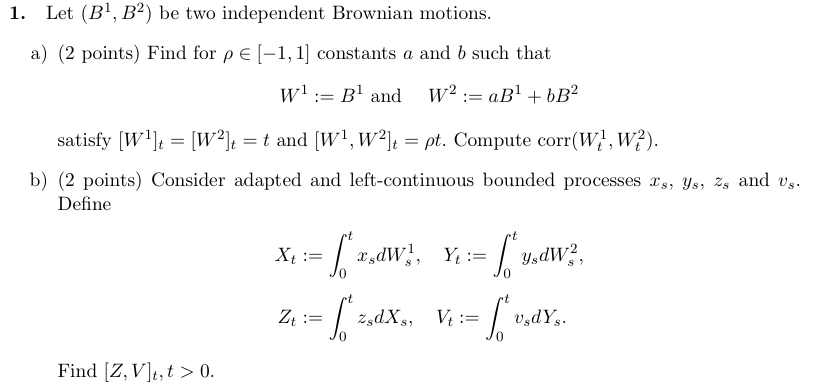
\includegraphics[width=\textwidth]{ex1.png}

Since the Feynman-Kac Formula works in both directions,
we choose to show that from the conditional expectation one can
derive the PDE.

\begin{align*}
	F \lb t, V_t \rb &= E^Q_{\lb t, V_t \rb} \lb \int_t^T e^{-r(s-t)} d(V_s) ds \rb \\
	\text{adding to both sides } & E^Q_{\lb t, V_t \rb} \lb \int_0^t e^{-r(s-0)} d(V_s) ds \rb\\
F \lb t, V_t \rb + E^Q_{\lb t, V_t \rb} \lb \int_0^t e^{-r(s-0)} d(V_s) ds \rb &=
E^Q_{\lb t, V_t \rb} \lb \underbrace{\int_0^T e^{-r(s-0)} d(V_s) ds}_{Z} \rb 
\end{align*}
since $Z$ does not debend on t we can conclude from the properties of conditional expectation that
it is a martingale hance the left hand side is also a martingale.
We therefore can apply Ito's Lemma to the left hand side and end up with the PDE given the condition
that $F(T,v)=0$.


\end{document}
